Zur Bestimmung der Dämpfungskonstante wird mit dem Oszilloskop für ein langes und ein kurzes Kabel eine FFT eines Rechteckpulses durchgeführt. Die hier entstandenen Bilder sind in Abbildung \ref{fig:FFT} zu sehen. Die Position und Höhe der Peaks wird aus dem Datensatz extrahiert und sind in Tabelle \ref{tab:DaempfungWerteB} zu sehen.
\begin{figure}[h]
	\centering
	\begin{subfigure}{0.495\textwidth}
		\centering
		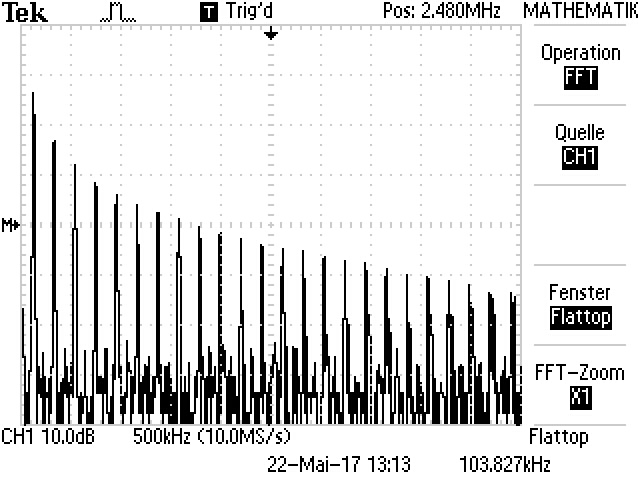
\includegraphics[width=0.9\textwidth]{Oszilloskop/DaempfungLang/F0042TEK.JPG}
		\subcaption{Langes Kabel}
		\label{fig:FFTLang}
	\end{subfigure}
	\begin{subfigure}{0.495\textwidth}
		\centering
		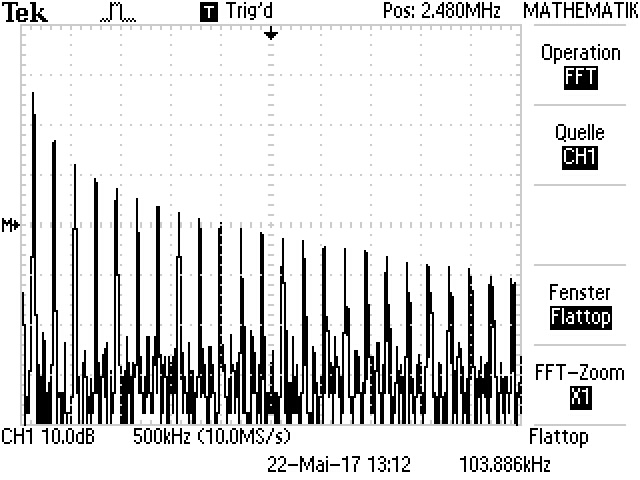
\includegraphics[width=0.9\textwidth]{Oszilloskop/DaempfungKurz/F0041TEK.JPG}
		\subcaption{Kurzes Kabel}
		\label{fig:FFTKurz}
	\end{subfigure}
	\caption{Oszilloskop-Bilder der FFT}
	\label{fig:FFT}
\end{figure} \\
Da ein ungerades Rechtecksignal betrachtet wird, sind die $\omega_n$ ungerade Vielfache der Grundfrequenz $\omega_0$. Es wird die Vermutung aufgestellt, dass das Oszilloskop die Fouriertransformierte dabei mit
\begin{align}\label{eq:Vermutung}
	P = \ln\left(\frac{U(\omega)}{U_0}\right)
\end{align}
normiert. Die Fourierkoeffizienten und die Fouriertransformierte eines ungeraden Rechtecksignals sind
\begin{align*}
	A_n &=\frac{4U_0}{\pi(2n+1)} = \frac{A_0}{2n+1} \quad, \\
	U(\omega) &= \sum_{n=0}^{\infty}A_n\delta(\omega-\omega_0(2n+1)) \quad.
\end{align*}
Die Amplituden, die das Oszilloskop mit der FFT darstellt können demnach auch durch die Fourierkoeffizienten ausgedrückt werden:
\begin{align}\label{eq:P}
	P_n = \ln\left(\frac{A_n}{A_0}\right) &= \ln\left(\frac{\omega_0}{\omega_n}\right)\notag \\
	&= \ln\left(\frac{\omega_0}{\omega_n}\right)\si{\neper}\notag \quad\footnotemark \\
	&= 20\log_{10}\left(\frac{\omega_0}{\omega_n}\right)\si{\deci\bel} \quad.
\end{align}
Die Grundfrequenz ist dabei
\begin{align*}
	\omega_0 = \frac{\omega(A_n)}{2n+1} = \input{Daempfung/build/omega0} \quad.
\end{align*}
Abbildung \ref{eq:DaempfungB} zeigt diese Amplituden zusammen mit den aus den Messwerten und bestätigt die Vermutung \eqref{eq:Vermutung}, wenn bedacht wird, dass auch beim kurzen Kabel Verluste z.B. an den Verbindungsstücken auftauchen. \footnotetext{\si{\neper} ist eine Einheit, die das Verhältnis von zwei Werten angibt. Sie kann hier einfach hinzugefügt werden, da \SI{1}{\neper} = 1.}
\begin{figure}[h]
	\centering
	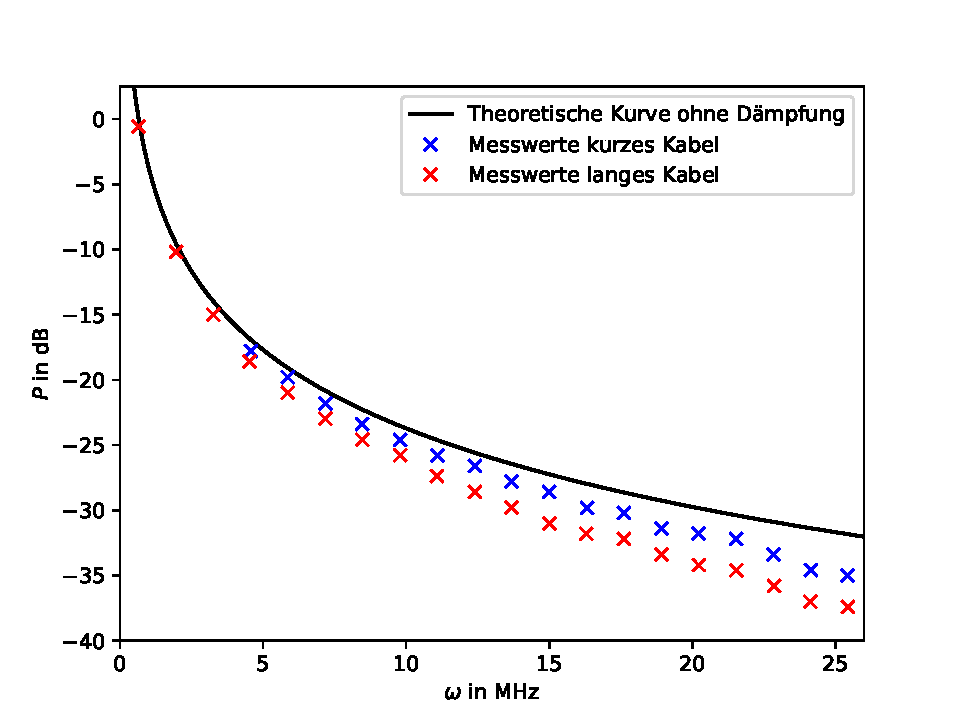
\includegraphics[width=0.8\textwidth]{Daempfung/build/PlotB.pdf}
	\caption{Aus dem Oszilloskop-Datensatz extrahierte Werte der Peaks mit der theoretischen Kurve aus \eqref{eq:P}}
	\label{fig:PlotDaempfungB}
\end{figure} \\
Die Dämpfungskonstante kann nun wie folgt berechnet werden
\begin{align}\label{eq:DaempfungB}
	P_{n,\text{Lang}}-P_{n,\text{Kurz}} &= \ln\left(\frac{U_{n,\text{Lang}}(\omega)}{U_0}\right) - \ln\left(\frac{U_{n,\text{Kurz}}(\omega)}{U_0}\right)\notag \\
	&= \ln\left(\frac{U_{n,\text{Lang}}(\omega)}{U_0}\right) - \ln\left(\frac{U_{n,\text{Kurz}}(\omega)}{U_0}\right)\si{\neper}\notag \\
	&= 20\cdot\log_{10}\left(\frac{U_{n,\text{Lang}}(\omega)}{U_{n,\text{Kurz}}(\omega)}\right)\si{\deci\bel}\notag \\
	&= 20\cdot\log_{10}\left(\exp(-\alpha L)\right)\si{\deci\bel}\notag \\
	&= -20\cdot\alpha\cdot L\cdot\log_{10}e\ \si{\deci\bel}\notag \\
	\Leftrightarrow\quad \alpha &= \frac{P_\text{Lang}-P_\text{Kurz}}{20\cdot L\cdot\log_{10}e\ \si{\deci\bel}} \quad.
\end{align}
Die  Werte für die Dämpfungskonstante sind in Tabelle \ref{tab:DaempfungWerteB} abgebildet. Die Mittelung ergibt
\begin{align}
	\alpha = \SI{3.64+-0.42}{\per\kilo\meter}
 \quad.
\end{align}
\begin{table}
    \centering
    \caption{Frequenz $\omega$ und Betrag der Amplitude $P$ der Peaks in der FFT für das kurze und das lange Kabel, sowie mit \eqref{eq:DaempfungB} berechnete Dämpfung}
    \label{tab:DaempfungWerteB}
    \sisetup{parse-numbers=false}
    \begin{tabular}{
	S[table-format=2.3]
	S[table-format=2.2]
	S[table-format=2.3]
	S[table-format=2.2]
	S[table-format=2.2]
	}
	\toprule
	{$\omega_\text{Kurz} \ \mathrm{in} \ \si{\mega\hertz}$}		& {$|P_\text{Kurz}| \ \mathrm{in} \ \si{\deci\bel}$}		& 
	{$\omega_\text{Lang} \ \mathrm{in} \ \si{\mega\hertz}$}		& {$|P_\text{Lang}| \ \mathrm{in} \ \si{\deci\bel}$}		& 
	{$\alpha \ \mathrm{in} \ \si{\per\kilo\meter}$}		\\ 
	\midrule
    0.644  & 0.59  & 0.644  & 0.59  & -0.00 \\
1.963  & 10.19 & 1.963  & 10.19 & -0.00 \\
3.252  & 14.99 & 3.252  & 14.99 & -0.00 \\
4.571  & 17.79 & 4.541  & 18.59 & 1.84  \\
5.860  & 19.79 & 5.860  & 20.99 & 2.76  \\
7.179  & 21.79 & 7.179  & 22.99 & 2.76  \\
8.468  & 23.39 & 8.468  & 24.59 & 2.76  \\
9.787  & 24.59 & 9.787  & 25.79 & 2.76  \\
11.106 & 25.79 & 11.075 & 27.39 & 3.68  \\
12.395 & 26.59 & 12.395 & 28.59 & 4.61  \\
13.683 & 27.79 & 13.683 & 29.79 & 4.61  \\
15.002 & 28.59 & 15.002 & 30.99 & 5.53  \\
16.322 & 29.79 & 16.291 & 31.79 & 4.61  \\
17.610 & 30.19 & 17.610 & 32.19 & 4.61  \\
18.929 & 31.39 & 18.929 & 33.39 & 4.61  \\
20.218 & 31.79 & 20.218 & 34.19 & 5.53  \\
21.537 & 32.19 & 21.537 & 34.59 & 5.53  \\
22.826 & 33.39 & 22.856 & 35.79 & 5.53  \\
24.145 & 34.59 & 24.114 & 36.99 & 5.53  \\
25.433 & 34.99 & 25.433 & 37.39 & 5.53  \\

    \bottomrule
    \end{tabular}
    \end{table}

